\documentclass[letterpaper,12pt,fleqn]{article}
\usepackage{matharticle}
\pagestyle{plain}

\newcommand{\red}[1]{\textcolor{red}{#1}}

\begin{document}

\begin{center}
  \large Math-42 Worksheet \#2

  \textbf{Applications of Propositional Logic}
\end{center}

\vspace{0.5in}

\begin{enumerate}[left=0in,itemsep=0.5in]
\item Consider the following compound propositions describing you visit to the DMV:
  \begin{itemize}
  \item You can wait in line if and only if you completed your paperwork online.
  \item If you completed your paperwork online then you can get your new driver's license.
  \item You cannot get a new driver's license or you cannot wait in line.
  \item You cannot wait in line implies you did not complete your paperwork online.
  \item You completed your paperwork online.
  \end{itemize}
  \begin{enumerate}
  \item Identify the simple propositions using \(p\), \(q\), and \(r\) as variables.
  \item Construct a system of logic equations using the variables that you assigned to the simple propositions.
  \item Determine if this system is consistent.  If not, then explain why.
  \end{enumerate}

\item You are traveling in Raymond Smullyan's land of knights and knaves.  Remember that knights always tell the
  truth (i.e., make a true statement) and knaves always lie (i.e., make a false statement).  You come upon two
  people, call them \(A\) and \(B\).  \(A\) says: ``If I am a knight then he is a knave.''  \(B\) says nothing.
  Determine whether each persons is either a knave or a knight.  Remember, if you start with person \(A\), you
  must examine both cases: \(A\) is a knight or \(A\) is not a knight (a knave).  Hint: when is a conditional
  true and when is it false?

\item We learned how to build a truth table from a logic equation last time.  But what if we are given the
  results of a truth table and are asked to reconstruct a logic equation?  For example, if you are given the
  truth table:
  \[\begin{array}{ccc|c}
  p & q & r & f \\
  \hline
  F & F & F & T \\
  F & F & T & F \\
  F & T & F & F \\
  F & T & T & T \\
  T & F & F & T \\
  T & F & T & F \\
  T & T & F & F \\
  T & T & T & F
  \end{array}\]
  How can you construct the logic equation for \(f\)?  One way is to construct the so-called \emph{canonical form}
  of \(f\).  In the canonical form, each true line in the truth table is represented by a term in an \emph{or}.
  Each term contains each variable in an \emph{and}.  If the variable value in the corresponding row is false then
  the negated form of the variable is used.
  \begin{enumerate}
  \item Start by identifying all of the rows where \(f\) is true.
  \item One of the rows that you should have identified is row \(1\), where \(p\), \(q\), and \(r\) are all false.
    Thus, the term for that row is \(\bar{p}\bar{q}\bar{r}\).  Construct the terms for the other rows.
  \item Or all of your terms together in order to get the final logic equation for \(f\).
  \end{enumerate}
  Note that the canonical form is not always the most simple expression for a logic equation.  There are
  simplification techniques (e.g., Boolean logic and Karnaugh maps), but we will study those techniques later as
  time permits.

\item The goal of this next exercise is to design a \(1\)-bit binary adder, similar to what would be found in the
  CPU of a computer.  These adders are chained together so that binary numbers of various bit lengths can be added
  together.  Recall that when binary numbers (base-\(2\)) are added, we use the same algorithm as when we add
  decimal (base-\(10\)) numbers: added each column (digit) to produce a sum and a possible carry to the next
  column.  For example, to add the binary numbers \(111\) and \(011\), we would do something like the following:
  \[\begin{array}{c ccc}
  \red{1} & \red{1} & \red{1} & \\
    & 1 & 1 & 1 \\
  + & 0 & 1 & 1 \\
  \hline
  1 & 0 & 1 & 0
  \end{array}\]

  Conceptually, the adder can be viewed as follows:

  \bigskip

  \begin{center}
    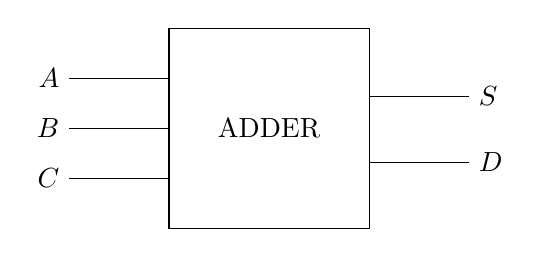
\begin{tikzpicture}
      \draw (0,0) rectangle (1in, 1in);
      \node at (0.5in,0.5in) {ADDER};
      \draw (0,0.75in) -- (-0.5in, 0.75in) node [left] {\(A\)};
      \draw (0,0.5in) -- (-0.5in, 0.5in) node [left] {\(B\)};
      \draw (0,0.25in) -- (-0.5in, 0.25in) node [left] {\(C\)};
      \draw (1in,0.33in) -- (1.5in,0.33in) node [right] {\(D\)};
      \draw (1in,0.66in) -- (1.5in,0.66in) node [right] {\(S\)};
    \end{tikzpicture}
  \end{center}

  \(A\) and \(B\) are the two bits to be added, \(C\) is the carry in from the previous adder, \(S\) is the sum,
  and \(D\) is the carry out to the next adder.
  \begin{enumerate}
  \item Construct a truth table (using \(0\) and \(1\) instead of \(F\) and \(T\)) that has \(A\), \(B\), and
    \(C\) as inputs and \(S\) and \(D\) as outputs.
  \item Determine the canonical forms for the logic equations for \(S\) and \(D\).
  \item Assuming that you have some \(3\)-input AND gates, some \(4\)-input OR gates, and some invertors (NOT
    gates), draw the logic circuits for \(S\) and \(D\).
  \end{enumerate}
\end{enumerate}

\end{document}
